% Bloque independiente. Sustituir los campos por evidencia de su proyecto.
\bloque{\personaDos}
\section{gRPC}
\begin{frame}{gRPC: un contrato, dos extremos}\relax
	{\bfseries El servicio se define una sola vez en un archivo \texttt{.proto}; de ese contrato se genera el código del cliente y del servidor.\par}
	\medskip
	\centering
	\begin{tikzpicture}[font=\small]
		\node[nodo] (p) at (4.5,1.8) {\texttt{turnos.proto}\\contrato};
		\node[nodo] (c) at (0,0) {Cliente\\\textbf{stub} generado};
		\node[nodo] (s) at (9,0) {Servidor\\implementación};
		\draw[enlace,-Stealth,dashed] (p)--node[above left,font=\footnotesize]{genera}(c);
		\draw[enlace,-Stealth,dashed] (p)--node[above right,font=\footnotesize]{genera}(s);
		\draw[enlace] (c)--node[below,font=\footnotesize]{HTTP/2 + Protocol Buffers (binario)}(s);
	\end{tikzpicture}
	\par\smallskip
	\raggedright
	{\small El cliente y el servidor pueden estar en lenguajes distintos: solo comparten el contrato.}
	{\footnotesize Fuente: \cite{kaminski2023}.}
\end{frame}

\begin{frame}{Ejemplo: consulta de turno por placa}\relax
	\small
	\textbf{Contrato}\quad{\scriptsize\texttt{rpc ConsultarTurno(ConsultaTurnoRequest) returns (ConsultaTurnoResponse)}}\par
	\smallskip
	\textbf{Entrada}\quad placa \texttt{GSA-1234} \qquad \textbf{Salida}\quad turno el 2026-11-25 09:00, \texttt{CONFIRMADO}\par
	\smallskip
	\textbf{Llamada}\quad unaria y bloqueante, con un \emph{deadline} de 3 segundos.\par
	\smallskip
	\centering
	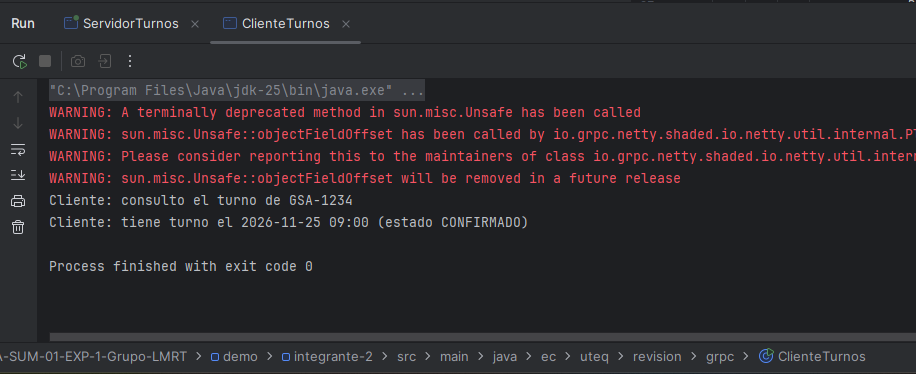
\includegraphics[width=.9\linewidth,height=.5\textheight,keepaspectratio]{../evidencias/integrante-2/demo-grpc/01-confirmado.png}
\end{frame}

\begin{frame}{\proyectoDos · arquitectura propuesta (vista parcial)}\relax
{\footnotesize\textbf{Actualmente}\quad El CRTVMV atiende cada vehículo en cinco puestos: guardia, recepción, recaudación, línea y digitación. El prototipo del PFC separa Inspecciones y Turnos y Pagos y los une por REST; p95 de 47,4 ms con 10 usuarios (medición local del equipo, 20/11/2026) \cite{rtvpfc2026}.}
\par\smallskip
\centering
\resizebox{.84\linewidth}{!}{% Diagrama propio de Allison Mera Jumbo, derivado del bosquejo a mano del 20-11-2026.
% Vista parcial del RTV: solo la autorización de inicio de inspección.
% Lo rojo es supuesto (gRPC), no implementado; hoy esa llamada es REST.
\begin{tikzpicture}[
  x=1cm,y=1cm,
  bloque/.style={draw=Azul!60,fill=Bruma,rounded corners=2pt,
    align=center,text width=2.6cm,minimum height=1.05cm,inner sep=4pt,font=\fontsize{9}{10.5}\selectfont},
  base/.style={draw=Azul!60,fill=white,rounded corners=2pt,align=center,text width=2.3cm,
    minimum height=.8cm,font=\fontsize{8.5}{10}\selectfont},
  flujo/.style={-{Stealth[length=2mm]},thick,draw=Azul},
  rotulo/.style={font=\fontsize{8}{9.5}\selectfont,align=center,text=Tinta}
]
\node[bloque,fill=white] (ins) at (0,0) {\textbf{Técnico inspector}\\o recepción};
\node[bloque] (insp) at (4.6,0) {\textbf{Inspecciones}\\Spring Boot\\stub gRPC};
\node[bloque] (tyP) at (11.6,0) {\textbf{Turnos y Pagos}\\Spring Boot\\servidor gRPC};
\node[base] (db1) at (4.6,-2.2) {PostgreSQL\\inspecciones};
\node[base] (db2) at (11.6,-2.2) {PostgreSQL\\turnos y pagos};
\draw[flujo] (ins.east) -- node[above,rotulo]{iniciar} (insp.west);
\draw[flujo,draw=Pendiente,very thick] ([yshift=2.5mm]insp.east) -- node[above=2pt,rotulo,text=Pendiente]{\textbf{gRPC}\\\texttt{AutorizarInspeccion}} ([yshift=2.5mm]tyP.west);
\draw[flujo,draw=Pendiente,very thick] ([yshift=-2.5mm]tyP.west) -- node[below=2pt,rotulo,text=Pendiente]{\texttt{autorizacion\_id}\\o código de estado} ([yshift=-2.5mm]insp.east);
\draw[flujo] (insp.south) -- node[right,rotulo]{JDBC} (db1.north);
\draw[flujo] (tyP.south) -- node[right,rotulo]{JDBC} (db2.north);
\node[rotulo,anchor=center] at (8.1,-2.2) {\textit{Hoy:} REST\\\texttt{POST /turnos/\{id\}/}\\\texttt{autorizaciones-inspeccion}};
\end{tikzpicture}}
\par\smallskip
\raggedright
{\footnotesize\textbf{Propuesta}\quad Llevar la autorización de inicio a gRPC unario: contrato \texttt{.proto} tipado, stub generado y códigos de estado estándar, con la misma clave de idempotencia.}
\end{frame}

\begin{frame}{Decisiones al distribuir el RTV (supuesto)}\relax
\small
\begin{tabularx}{\linewidth}{@{}lX@{}}
\toprule
Comunicación & gRPC unario y bloqueante con \emph{deadline} de 3 s: Inspecciones necesita la autorización antes de registrar el inicio.\\
Transparencias & \textbf{Ofrecida:} acceso, \texttt{AutorizarInspeccion} se llama como un método local. \textbf{Limitada:} fallos; el inspector vería \texttt{UNAVAILABLE} o \texttt{DEADLINE\_EXCEEDED} (probado en la demo).\\
CAP & Una instancia por servicio y bases separadas. Si se corta el enlace: consistencia, no se inicia una inspección sin autorización.\\
PACELC & Red sana: consistencia sobre latencia; se guarda una sola autorización por turno. Mediría el p95 con gRPC y lo compararía con los 47,4 ms de REST.\\
\bottomrule
\end{tabularx}
\end{frame}

\begin{frame}{Fallo hipotético y lección para el RTV}\relax
\small
\textbf{Escenario}\quad Turnos y Pagos guarda la autorización, pero la respuesta no llega antes del \emph{deadline}.\par\smallskip
\textbf{Causa raíz}\quad El \emph{deadline} vencido no cancela lo que el servidor ya escribió \cite{grpcdeadlines}.\par\smallskip
\textbf{Respuesta}\quad Inspecciones recibe \texttt{DEADLINE\_EXCEEDED} y reintenta con la misma clave; el servidor devuelve la autorización original.\par\smallskip
\textbf{Comparación}\quad Stripe guarda el resultado de cada clave de idempotencia y lo devuelve en los reintentos \cite{stripeidempotency}. Compromiso: persistir las claves.\par\smallskip
\textbf{Lección}\quad Primero, la clave de idempotencia en el contrato. Prueba pendiente: demorar el servidor más de 3 s, reintentar y contar una sola autorización.\par
\end{frame}